% REV00 Tue 04 May 2021 13:55:16 WIB
% START Tue 04 May 2021 13:55:16 WIB

\chapter{XXX}

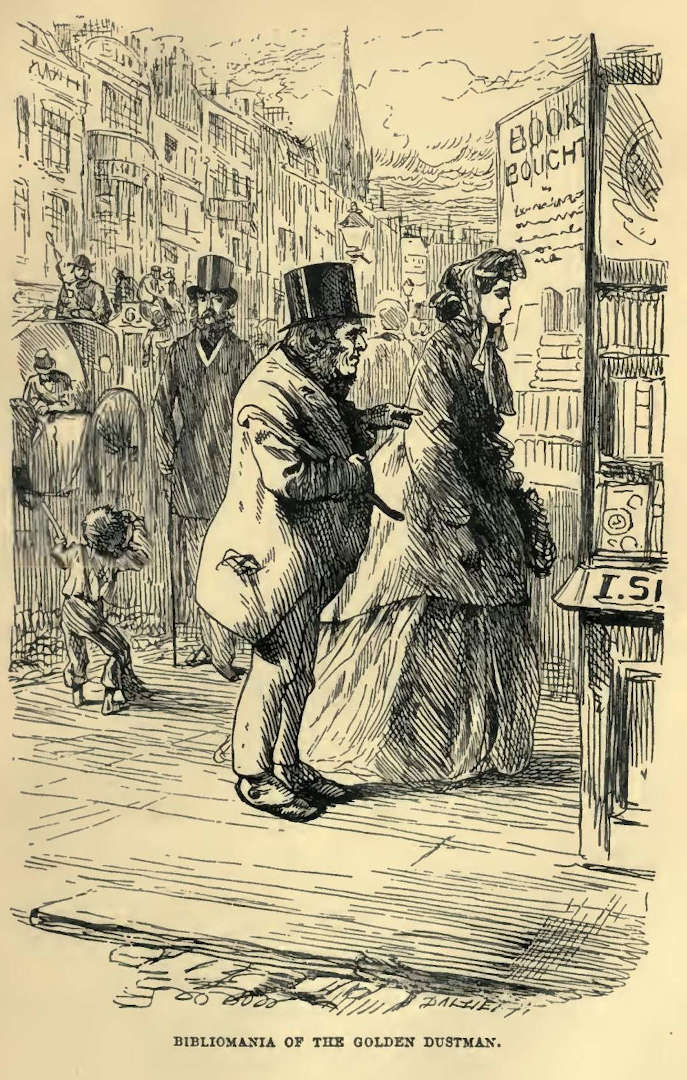
\includegraphics[scale=2.3]{03-05-01}

Chapter 8

A FEW GRAINS OF PEPPER


The dolls’ dressmaker went no more to the business-premises of Pubsey
and Co. in St Mary Axe, after chance had disclosed to her (as she
supposed) the flinty and hypocritical character of Mr Riah. She often
moralized over her work on the tricks and the manners of that venerable
cheat, but made her little purchases elsewhere, and lived a secluded
life. After much consultation with herself, she decided not to put
Lizzie Hexam on her guard against the old man, arguing that the
disappointment of finding him out would come upon her quite soon enough.
Therefore, in her communication with her friend by letter, she was
silent on this theme, and principally dilated on the backslidings of her
bad child, who every day grew worse and worse.

‘You wicked old boy,’ Miss Wren would say to him, with a menacing
forefinger, ‘you’ll force me to run away from you, after all, you will;
and then you’ll shake to bits, and there’ll be nobody to pick up the
pieces!’

At this foreshadowing of a desolate decease, the wicked old boy would
whine and whimper, and would sit shaking himself into the lowest of low
spirits, until such time as he could shake himself out of the house and
shake another threepennyworth into himself. But dead drunk or dead
sober (he had come to such a pass that he was least alive in the latter
state), it was always on the conscience of the paralytic scarecrow that
he had betrayed his sharp parent for sixty threepennyworths of rum,
which were all gone, and that her sharpness would infallibly detect his
having done it, sooner or later. All things considered therefore, and
addition made of the state of his body to the state of his mind, the bed
on which Mr Dolls reposed was a bed of roses from which the flowers
and leaves had entirely faded, leaving him to lie upon the thorns and
stalks.

On a certain day, Miss Wren was alone at her work, with the house-door
set open for coolness, and was trolling in a small sweet voice a
mournful little song which might have been the song of the doll she was
dressing, bemoaning the brittleness and meltability of wax, when whom
should she descry standing on the pavement, looking in at her, but Mr
Fledgeby.

‘I thought it was you?’ said Fledgeby, coming up the two steps.

‘Did you?’ Miss Wren retorted. ‘And I thought it was you, young man.
Quite a coincidence. You’re not mistaken, and I’m not mistaken. How
clever we are!’

‘Well, and how are you?’ said Fledgeby.

‘I am pretty much as usual, sir,’ replied Miss Wren. ‘A very unfortunate
parent, worried out of my life and senses by a very bad child.’

Fledgeby’s small eyes opened so wide that they might have passed for
ordinary-sized eyes, as he stared about him for the very young person
whom he supposed to be in question.

‘But you’re not a parent,’ said Miss Wren, ‘and consequently it’s of no
use talking to you upon a family subject.--To what am I to attribute the
honour and favour?’

‘To a wish to improve your acquaintance,’ Mr Fledgeby replied.

Miss Wren, stopping to bite her thread, looked at him very knowingly.

‘We never meet now,’ said Fledgeby; ‘do we?’

‘No,’ said Miss Wren, chopping off the word.

‘So I had a mind,’ pursued Fledgeby, ‘to come and have a talk with you
about our dodging friend, the child of Israel.’

‘So HE gave you my address; did he?’ asked Miss Wren.

‘I got it out of him,’ said Fledgeby, with a stammer.

‘You seem to see a good deal of him,’ remarked Miss Wren, with shrewd
distrust. ‘A good deal of him you seem to see, considering.’

‘Yes, I do,’ said Fledgeby. ‘Considering.’

‘Haven’t you,’ inquired the dressmaker, bending over the doll on which
her art was being exercised, ‘done interceding with him yet?’

‘No,’ said Fledgeby, shaking his head.

‘La! Been interceding with him all this time, and sticking to him
still?’ said Miss Wren, busy with her work.

‘Sticking to him is the word,’ said Fledgeby.

Miss Wren pursued her occupation with a concentrated air, and asked,
after an interval of silent industry:

‘Are you in the army?’

‘Not exactly,’ said Fledgeby, rather flattered by the question.

‘Navy?’ asked Miss Wren.

‘N--no,’ said Fledgeby. He qualified these two negatives, as if he were
not absolutely in either service, but was almost in both.

‘What are you then?’ demanded Miss Wren.

‘I am a gentleman, I am,’ said Fledgeby.

‘Oh!’ assented Jenny, screwing up her mouth with an appearance of
conviction. ‘Yes, to be sure! That accounts for your having so much
time to give to interceding. But only to think how kind and friendly a
gentleman you must be!’

Mr Fledgeby found that he was skating round a board marked Dangerous,
and had better cut out a fresh track. ‘Let’s get back to the dodgerest
of the dodgers,’ said he. ‘What’s he up to in the case of your friend
the handsome gal? He must have some object. What’s his object?’

‘Cannot undertake to say, sir, I am sure!’ returned Miss Wren,
composedly.

‘He won’t acknowledge where she’s gone,’ said Fledgeby; ‘and I have
a fancy that I should like to have another look at her. Now I know he
knows where she is gone.’

‘Cannot undertake to say, sir, I am sure!’ Miss Wren again rejoined.

‘And you know where she is gone,’ hazarded Fledgeby.

‘Cannot undertake to say, sir, really,’ replied Miss Wren.

The quaint little chin met Mr Fledgeby’s gaze with such a baffling
hitch, that that agreeable gentleman was for some time at a loss how to
resume his fascinating part in the dialogue. At length he said:

‘Miss Jenny!--That’s your name, if I don’t mistake?’

‘Probably you don’t mistake, sir,’ was Miss Wren’s cool answer; ‘because
you had it on the best authority. Mine, you know.’

‘Miss Jenny! Instead of coming up and being dead, let’s come out and
look alive. It’ll pay better, I assure you,’ said Fledgeby, bestowing
an inveigling twinkle or two upon the dressmaker. ‘You’ll find it pay
better.’

‘Perhaps,’ said Miss Jenny, holding out her doll at arm’s length, and
critically contemplating the effect of her art with her scissors on her
lips and her head thrown back, as if her interest lay there, and not in
the conversation; ‘perhaps you’ll explain your meaning, young man, which
is Greek to me.--You must have another touch of blue in your trimming,
my dear.’ Having addressed the last remark to her fair client, Miss
Wren proceeded to snip at some blue fragments that lay before her, among
fragments of all colours, and to thread a needle from a skein of blue
silk.

‘Look here,’ said Fledgeby.--‘Are you attending?’

‘I am attending, sir,’ replied Miss Wren, without the slightest
appearance of so doing. ‘Another touch of blue in your trimming, my
dear.’

‘Well, look here,’ said Fledgeby, rather discouraged by the
circumstances under which he found himself pursuing the conversation.
‘If you’re attending--’

[‘Light blue, my sweet young lady,’ remarked Miss Wren, in a sprightly
tone, ‘being best suited to your fair complexion and your flaxen
curls.’)

‘I say, if you’re attending,’ proceeded Fledgeby, ‘it’ll pay better in
this way. It’ll lead in a roundabout manner to your buying damage and
waste of Pubsey and Co. at a nominal price, or even getting it for
nothing.’

‘Aha!’ thought the dressmaker. ‘But you are not so roundabout, Little
Eyes, that I don’t notice your answering for Pubsey and Co. after all!
Little Eyes, Little Eyes, you’re too cunning by half.’

‘And I take it for granted,’ pursued Fledgeby, ‘that to get the most of
your materials for nothing would be well worth your while, Miss Jenny?’

‘You may take it for granted,’ returned the dressmaker with many knowing
nods, ‘that it’s always well worth my while to make money.’

‘Now,’ said Fledgeby approvingly, ‘you’re answering to a sensible
purpose. Now, you’re coming out and looking alive! So I make so free,
Miss Jenny, as to offer the remark, that you and Judah were too thick
together to last. You can’t come to be intimate with such a deep file
as Judah without beginning to see a little way into him, you know,’ said
Fledgeby with a wink.

‘I must own,’ returned the dressmaker, with her eyes upon her work,
‘that we are not good friends at present.’

‘I know you’re not good friends at present,’ said Fledgeby. ‘I know all
about it. I should like to pay off Judah, by not letting him have his
own deep way in everything. In most things he’ll get it by hook or
by crook, but--hang it all!--don’t let him have his own deep way in
everything. That’s too much.’ Mr Fledgeby said this with some display of
indignant warmth, as if he was counsel in the cause for Virtue.

‘How can I prevent his having his own way?’ began the dressmaker.

‘Deep way, I called it,’ said Fledgeby.

‘--His own deep way, in anything?’

‘I’ll tell you,’ said Fledgeby. ‘I like to hear you ask it, because
it’s looking alive. It’s what I should expect to find in one of your
sagacious understanding. Now, candidly.’

‘Eh?’ cried Miss Jenny.

‘I said, now candidly,’ Mr Fledgeby explained, a little put out.

‘Oh-h!’

‘I should be glad to countermine him, respecting the handsome gal, your
friend. He means something there. You may depend upon it, Judah means
something there. He has a motive, and of course his motive is a dark
motive. Now, whatever his motive is, it’s necessary to his motive’--Mr
Fledgeby’s constructive powers were not equal to the avoidance of some
tautology here--‘that it should be kept from me, what he has done with
her. So I put it to you, who know: What HAS he done with her? I ask no
more. And is that asking much, when you understand that it will pay?’

Miss Jenny Wren, who had cast her eyes upon the bench again after her
last interruption, sat looking at it, needle in hand but not working,
for some moments. She then briskly resumed her work, and said with a
sidelong glance of her eyes and chin at Mr Fledgeby:

‘Where d’ye live?’

‘Albany, Piccadilly,’ replied Fledgeby.

‘When are you at home?’

‘When you like.’

‘Breakfast-time?’ said Jenny, in her abruptest and shortest manner.

‘No better time in the day,’ said Fledgeby.

‘I’ll look in upon you to-morrow, young man. Those two ladies,’ pointing
to dolls, ‘have an appointment in Bond Street at ten precisely. When
I’ve dropped ‘em there, I’ll drive round to you.’ With a weird little
laugh, Miss Jenny pointed to her crutch-stick as her equipage.

‘This is looking alive indeed!’ cried Fledgeby, rising.

‘Mark you! I promise you nothing,’ said the dolls’ dressmaker, dabbing
two dabs at him with her needle, as if she put out both his eyes.

‘No no. I understand,’ returned Fledgeby. ‘The damage and waste question
shall be settled first. It shall be made to pay; don’t you be afraid.
Good-day, Miss Jenny.’

‘Good-day, young man.’

Mr Fledgeby’s prepossessing form withdrew itself; and the little
dressmaker, clipping and snipping and stitching, and stitching and
snipping and clipping, fell to work at a great rate; musing and
muttering all the time.

‘Misty, misty, misty. Can’t make it out. Little Eyes and the wolf in a
conspiracy? Or Little Eyes and the wolf against one another? Can’t make
it out. My poor Lizzie, have they both designs against you, either way?
Can’t make it out. Is Little Eyes Pubsey, and the wolf Co? Can’t make it
out. Pubsey true to Co, and Co to Pubsey? Pubsey false to Co, and Co to
Pubsey? Can’t make it out. What said Little Eyes? “Now, candidly?”
 Ah! However the cat jumps, HE’S a liar. That’s all I can make out at
present; but you may go to bed in the Albany, Piccadilly, with THAT for
your pillow, young man!’ Thereupon, the little dressmaker again dabbed
out his eyes separately, and making a loop in the air of her thread and
deftly catching it into a knot with her needle, seemed to bowstring him
into the bargain.

For the terrors undergone by Mr Dolls that evening when his little
parent sat profoundly meditating over her work, and when he imagined
himself found out, as often as she changed her attitude, or turned her
eyes towards him, there is no adequate name. Moreover it was her habit
to shake her head at that wretched old boy whenever she caught his eye
as he shivered and shook. What are popularly called ‘the trembles’ being
in full force upon him that evening, and likewise what are popularly
called ‘the horrors,’ he had a very bad time of it; which was not
made better by his being so remorseful as frequently to moan ‘Sixty
threepennorths.’ This imperfect sentence not being at all intelligible
as a confession, but sounding like a Gargantuan order for a dram,
brought him into new difficulties by occasioning his parent to pounce
at him in a more than usually snappish manner, and to overwhelm him with
bitter reproaches.

What was a bad time for Mr Dolls, could not fail to be a bad time for
the dolls’ dressmaker. However, she was on the alert next morning, and
drove to Bond Street, and set down the two ladies punctually, and then
directed her equipage to conduct her to the Albany. Arrived at the
doorway of the house in which Mr Fledgeby’s chambers were, she found a
lady standing there in a travelling dress, holding in her hand--of all
things in the world--a gentleman’s hat.

‘You want some one?’ said the lady in a stern manner.

‘I am going up stairs to Mr Fledgeby’s.’

‘You cannot do that at this moment. There is a gentleman with him. I am
waiting for the gentleman. His business with Mr Fledgeby will very soon
be transacted, and then you can go up. Until the gentleman comes down,
you must wait here.’

While speaking, and afterwards, the lady kept watchfully between her and
the staircase, as if prepared to oppose her going up, by force. The
lady being of a stature to stop her with a hand, and looking mightily
determined, the dressmaker stood still.

‘Well? Why do you listen?’ asked the lady.

‘I am not listening,’ said the dressmaker.

‘What do you hear?’ asked the lady, altering her phrase.

‘Is it a kind of a spluttering somewhere?’ said the dressmaker, with an
inquiring look.

‘Mr Fledgeby in his shower-bath, perhaps,’ remarked the lady, smiling.

‘And somebody’s beating a carpet, I think?’

‘Mr Fledgeby’s carpet, I dare say,’ replied the smiling lady.

Miss Wren had a reasonably good eye for smiles, being well accustomed
to them on the part of her young friends, though their smiles mostly ran
smaller than in nature. But she had never seen so singular a smile
as that upon this lady’s face. It twitched her nostrils open in a
remarkable manner, and contracted her lips and eyebrows. It was a smile
of enjoyment too, though of such a fierce kind that Miss Wren thought
she would rather not enjoy herself than do it in that way.

‘Well!’ said the lady, watching her. ‘What now?’

‘I hope there’s nothing the matter!’ said the dressmaker.

‘Where?’ inquired the lady.

‘I don’t know where,’ said Miss Wren, staring about her. ‘But I never
heard such odd noises. Don’t you think I had better call somebody?’

‘I think you had better not,’ returned the lady with a significant
frown, and drawing closer.

On this hint, the dressmaker relinquished the idea, and stood looking
at the lady as hard as the lady looked at her. Meanwhile the dressmaker
listened with amazement to the odd noises which still continued, and the
lady listened too, but with a coolness in which there was no trace of
amazement.

Soon afterwards, came a slamming and banging of doors; and then came
running down stairs, a gentleman with whiskers, and out of breath, who
seemed to be red-hot.

‘Is your business done, Alfred?’ inquired the lady.

‘Very thoroughly done,’ replied the gentleman, as he took his hat from
her.

‘You can go up to Mr Fledgeby as soon as you like,’ said the lady,
moving haughtily away.

‘Oh! And you can take these three pieces of stick with you,’ added the
gentleman politely, ‘and say, if you please, that they come from Mr
Alfred Lammle, with his compliments on leaving England. Mr Alfred
Lammle. Be so good as not to forget the name.’

The three pieces of stick were three broken and frayed fragments of a
stout lithe cane. Miss Jenny taking them wonderingly, and the gentleman
repeating with a grin, ‘Mr Alfred Lammle, if you’ll be so good.
Compliments, on leaving England,’ the lady and gentleman walked away
quite deliberately, and Miss Jenny and her crutch-stick went up stairs.
‘Lammle, Lammle, Lammle?’ Miss Jenny repeated as she panted from stair
to stair, ‘where have I heard that name? Lammle, Lammle? I know! Saint
Mary Axe!’

With a gleam of new intelligence in her sharp face, the dolls’
dressmaker pulled at Fledgeby’s bell. No one answered; but, from within
the chambers, there proceeded a continuous spluttering sound of a highly
singular and unintelligible nature.

‘Good gracious! Is Little Eyes choking?’ cried Miss Jenny.

Pulling at the bell again and getting no reply, she pushed the outer
door, and found it standing ajar. No one being visible on her opening it
wider, and the spluttering continuing, she took the liberty of opening
an inner door, and then beheld the extraordinary spectacle of Mr
Fledgeby in a shirt, a pair of Turkish trousers, and a Turkish cap,
rolling over and over on his own carpet, and spluttering wonderfully.

‘Oh Lord!’ gasped Mr Fledgeby. ‘Oh my eye! Stop thief! I am strangling.
Fire! Oh my eye! A glass of water. Give me a glass of water. Shut the
door. Murder! Oh Lord!’ And then rolled and spluttered more than ever.

Hurrying into another room, Miss Jenny got a glass of water, and brought
it for Fledgeby’s relief: who, gasping, spluttering, and rattling in his
throat betweenwhiles, drank some water, and laid his head faintly on her
arm.

‘Oh my eye!’ cried Fledgeby, struggling anew. ‘It’s salt and snuff. It’s
up my nose, and down my throat, and in my wind-pipe. Ugh! Ow! Ow! Ow!
Ah--h--h--h!’ And here, crowing fearfully, with his eyes starting out of
his head, appeared to be contending with every mortal disease incidental
to poultry.

‘And Oh my Eye, I’m so sore!’ cried Fledgeby, starting, over on his
back, in a spasmodic way that caused the dressmaker to retreat to the
wall. ‘Oh I smart so! Do put something to my back and arms, and legs and
shoulders. Ugh! It’s down my throat again and can’t come up. Ow! Ow! Ow!
Ah--h--h--h! Oh I smart so!’ Here Mr Fledgeby bounded up, and bounded
down, and went rolling over and over again.

The dolls’ dressmaker looked on until he rolled himself into a corner
with his Turkish slippers uppermost, and then, resolving in the first
place to address her ministration to the salt and snuff, gave him more
water and slapped his back. But, the latter application was by no means
a success, causing Mr Fledgeby to scream, and to cry out, ‘Oh my eye!
don’t slap me! I’m covered with weales and I smart so!’

However, he gradually ceased to choke and crow, saving at intervals,
and Miss Jenny got him into an easy-chair: where, with his eyes red and
watery, with his features swollen, and with some half-dozen livid bars
across his face, he presented a most rueful sight.

‘What ever possessed you to take salt and snuff, young man?’ inquired
Miss Jenny.

‘I didn’t take it,’ the dismal youth replied. ‘It was crammed into my
mouth.’

‘Who crammed it?’ asked Miss Jenny.

‘He did,’ answered Fledgeby. ‘The assassin. Lammle. He rubbed it into
my mouth and up my nose and down my throat--Ow! Ow! Ow! Ah--h--h--h!
Ugh!--to prevent my crying out, and then cruelly assaulted me.’

‘With this?’ asked Miss Jenny, showing the pieces of cane.

‘That’s the weapon,’ said Fledgeby, eyeing it with the air of an
acquaintance. ‘He broke it over me. Oh I smart so! How did you come by
it?’

‘When he ran down stairs and joined the lady he had left in the hall
with his hat’--Miss Jenny began.

‘Oh!’ groaned Mr Fledgeby, writhing, ‘she was holding his hat, was she?
I might have known she was in it.’

‘When he came down stairs and joined the lady who wouldn’t let me come
up, he gave me the pieces for you, and I was to say, “With Mr Alfred
Lammle’s compliments on his leaving England.”’ Miss Jenny said it with
such spiteful satisfaction, and such a hitch of her chin and eyes as
might have added to Mr Fledgeby’s miseries, if he could have noticed
either, in his bodily pain with his hand to his head.

‘Shall I go for the police?’ inquired Miss Jenny, with a nimble start
towards the door.

‘Stop! No, don’t!’ cried Fledgeby. ‘Don’t, please. We had better keep it
quiet. Will you be so good as shut the door? Oh I do smart so!’

In testimony of the extent to which he smarted, Mr Fledgeby came
wallowing out of the easy-chair, and took another roll on the carpet.

‘Now the door’s shut,’ said Mr Fledgeby, sitting up in anguish, with
his Turkish cap half on and half off, and the bars on his face getting
bluer, ‘do me the kindness to look at my back and shoulders. They must
be in an awful state, for I hadn’t got my dressing-gown on, when the
brute came rushing in. Cut my shirt away from the collar; there’s a pair
of scissors on that table. Oh!’ groaned Mr Fledgeby, with his hand to
his head again. ‘How I do smart, to be sure!’

‘There?’ inquired Miss Jenny, alluding to the back and shoulders.

‘Oh Lord, yes!’ moaned Fledgeby, rocking himself. ‘And all over!
Everywhere!’

The busy little dressmaker quickly snipped the shirt away, and laid
bare the results of as furious and sound a thrashing as even Mr Fledgeby
merited. ‘You may well smart, young man!’ exclaimed Miss Jenny. And
stealthily rubbed her little hands behind him, and poked a few exultant
pokes with her two forefingers over the crown of his head.

‘What do you think of vinegar and brown paper?’ inquired the suffering
Fledgeby, still rocking and moaning. ‘Does it look as if vinegar and
brown paper was the sort of application?’

‘Yes,’ said Miss Jenny, with a silent chuckle. ‘It looks as if it ought
to be Pickled.’

Mr Fledgeby collapsed under the word ‘Pickled,’ and groaned again.
‘My kitchen is on this floor,’ he said; ‘you’ll find brown paper in a
dresser-drawer there, and a bottle of vinegar on a shelf. Would you have
the kindness to make a few plasters and put ‘em on? It can’t be kept too
quiet.’

‘One, two--hum--five, six. You’ll want six,’ said the dress-maker.

‘There’s smart enough,’ whimpered Mr Fledgeby, groaning and writhing
again, ‘for sixty.’

Miss Jenny repaired to the kitchen, scissors in hand, found the brown
paper and found the vinegar, and skilfully cut out and steeped six
large plasters. When they were all lying ready on the dresser, an idea
occurred to her as she was about to gather them up.

‘I think,’ said Miss Jenny with a silent laugh, ‘he ought to have a
little pepper? Just a few grains? I think the young man’s tricks and
manners make a claim upon his friends for a little pepper?’

Mr Fledgeby’s evil star showing her the pepper-box on the chimneypiece,
she climbed upon a chair, and got it down, and sprinkled all the
plasters with a judicious hand. She then went back to Mr Fledgeby, and
stuck them all on him: Mr Fledgeby uttering a sharp howl as each was put
in its place.

‘There, young man!’ said the dolls’ dressmaker. ‘Now I hope you feel
pretty comfortable?’

Apparently, Mr Fledgeby did not, for he cried by way of answer, ‘Oh--h
how I do smart!’

Miss Jenny got his Persian gown upon him, extinguished his eyes
crookedly with his Persian cap, and helped him to his bed: upon which he
climbed groaning. ‘Business between you and me being out of the question
to-day, young man, and my time being precious,’ said Miss Jenny then,
‘I’ll make myself scarce. Are you comfortable now?’

‘Oh my eye!’ cried Mr Fledgeby. ‘No, I ain’t. Oh--h--h! how I do smart!’

The last thing Miss Jenny saw, as she looked back before closing the
room door, was Mr Fledgeby in the act of plunging and gambolling all
over his bed, like a porpoise or dolphin in its native element. She then
shut the bedroom door, and all the other doors, and going down stairs
and emerging from the Albany into the busy streets, took omnibus for
Saint Mary Axe: pressing on the road all the gaily-dressed ladies whom
she could see from the window, and making them unconscious lay-figures
for dolls, while she mentally cut them out and basted them.



